%\documentclass[iop]{emulateapj}
%\documentclass[12pt, preprint]{emulateapj}
\documentclass[12pt, onecolumn]{emulateapj}

\usepackage{amsmath}
%\usepackage{bibtex}
%\bibliographystyle{unsrtnat}

\usepackage{tikz}
\usetikzlibrary{shapes.geometric, arrows}
\usetikzlibrary{fit}

\tikzstyle{hyper} = [circle, text centered, draw=black]
\tikzstyle{param} = [circle, text centered, draw=black]
\tikzstyle{data} = [circle, text centered, draw=black, line width=2pt]
\tikzstyle{arrow} = [thick,->,>=stealth]
\tikzset{det/.style={insert path={ node {.} }}}

\newcommand{\myemail}{aimalz@nyu.edu}
\newcommand{\textul}{\underline}

%\slugcomment{}

\shorttitle{Propagating SNe misclassification probabilities into $H_{0}$}
\shortauthors{Malz}

\begin{document}

\title{Propagating supernova type misclassification probabilities through $H_{0}$ estimation: the fully probabilistic approach}

\author{A.I. Malz\altaffilmark{1}}
\author{Maryam Modjaz\altaffilmark{1}}
\author{Federica Bianco\altaffilmark{1}}
\altaffiltext{1}{CCPP}
\email{aimalz@nyu.edu}

\begin{abstract}
This document outlines a method for incorporating supernova type classification probabilities into calculations of the Hubble parameter $H(z)$ using a hierarchical Bayesian approach based on a probabilistic graphical model.
\end{abstract}

\keywords{}

\section{The problem}
\label{sec:intro}

Supernovae of type Ia (hereafter SNe Ia) serve as standardizable candles that can be used to obtain the redshift-dependent expansion rate of the universe $H(z)$ known as the Hubble parameter.  Ongoing and future photometric surveys will observe SNe Ia with irregular cadence and without spectroscopic confirmation, leading to large uncertainties in type classification and redshift estimation.  However, posterior probabilities on type and redshift may be obtained and used in calculations of the expansion rate.  

Current plans for utilizing classification and redshift probabilities involve imposing cuts to obtain a sample with a low contamination fraction and high completeness.  This approach unfortunately throws out information, excluding some SNe Ia and including some contaminants, such as type Ib/c supernovae (hereafter SNe Ib/c).  As an alternative, the set of joint posterior probabilities over type and redshift produced by a given survey may be used in full to calculate the posterior probability distribution over the Hubble parameter.  

\section{A proposed solution}
\label{sec:confrac}

Let us consider a simplified case in which the full sample of $N$ observed transients in a photometric survey are close enough in redshift that the Hubble parameter $H(z)$ is a constant $H_{0}$, which we shall call the Hubble constant.  The data $\{\textul{d}_{n}\}_{N}$ from this hypothetical survey consist of $N$ matrices $\textul{d}_{n}$ each comprised of a set of fluxes at $T_{n}$ lightcurve observation times in each of $F$ photometric filters specified by known parameters $\vec{f}$.  These represent samples of a true lightcurve specified by latent parameters $\vec{\ell}_{n}$ of the supernova at the location of the observer.  The lightcurve parameters are in turn determined by several other latent variables; its shape over time is determined by the properties $\vec{\alpha}_{m}$ associated with the type $s_{n}$ of supernova (out of $m$ possible types) in question, its magnitude is determined by its distance $r_{n}$ from the observer and the parameters determining its intrinsic luminosity $\vec{L}_{n}$, and its location in spectral space is determined by its redshift $z_{n}$.  There are some hyperparameters governing the distribution of each of these parameters; $H$ determines the relationship between $z_{n}$ and $r_{n}$, $D$ specifies the intrinsic density distribution of supernovae, and $S$ governs the distribution of supernova types.  This information may be summarized by the probabilistic graphical model of Fig. \ref{fig:pgm}.

\begin{figure}
\vspace{0.5cm}
\begin{center}
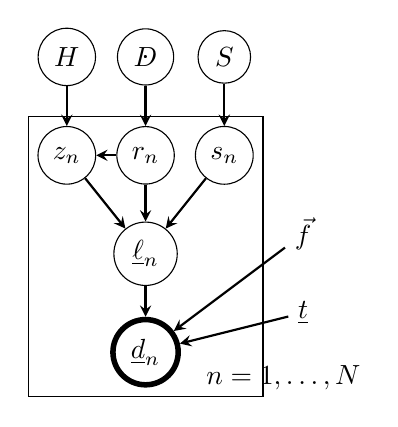
\begin{tikzpicture}[node distance=1cm]

\node (Hz) [hyper, xshift=-1cm] {$H$};
\node (Dr) [hyper] {$D$};
\node (Ss) [hyper, xshift=+1cm] {$S$};

\node (zn) [param, below of=Hz,yshift=-0.25cm] {$z_{n}$};
\node (rn) [param, below of=Dr,yshift=-0.25cm] {$r_{n}$};
\node (sn) [param, below of=Ss,yshift=-0.25cm] {$s_{n}$};

\node (lcn) [param, below of=rn,yshift=-0.25cm] {$\textul{\ell}_{n}$};

\node (dn) [data, below of=lcn,yshift=-0.25cm] {$\textul{d}_{n}$};

\node (f) [det,below of=sn,xshift=+1cm] {$\vec{f}$};
\node (t) [det,below of=f] {$\textul{t}$};

\node (survey) [draw=black,fit={(zn.west)(rn.north)(dn.south)(sn.east)}] {};
\node [xshift=1.75cm,yshift=0.25cm] at (survey.south) {$n=1,\dots,N$};

\draw [arrow] (Hz) -- (zn);
\draw [arrow] (Dr) -- (rn);
\draw [arrow] (Ss) -- (sn);

\draw [arrow] (rn) -- (zn);

\draw [arrow] (zn) -- (lcn);
\draw [arrow] (rn) -- (lcn);
\draw [arrow] (sn) -- (lcn);

\draw [arrow] (lcn) -- (dn);
\draw [arrow] (f) -- (dn);
\draw [arrow] (t) -- (dn);

\end{tikzpicture}
\caption{}
\label{fig:pgm}
\end{center}
\end{figure}

The model of Fig. \ref{fig:pgm} corresponds to the following equations for the posterior probability distribution $p(H|\{\textul{d}_{n}\}_{N})$.  

\begin{align*}
p(H|\{\textul{d}_{n}\}_{N}) &=\ p(\{\textul{d}_{n}\}_{N}|H)\frac{p(H)}{p(\{\textul{d}_{n}\}_{N})}\\
&\ p(\{\textul{d}_{n}\}_{N}|H)p(H)\\
&\propto\ \iint\ p(\{\textul{d}_{n}\}_{N}|H,D,S)\ p(H,D,S)\ dD\ dS\\
&\propto\ \iint\ p(\{\textul{d}_{n}\}_{N}|H,D,S)\ p(H)\ p(D)\ p(S)\ dD\ dS\\
&\propto\ \iint\ \left[\prod_{n=1}^{N}\ p(\textul{d}_{n}|H,D,S)\right]\ p(H)\ p(D)\ p(S)\ \ dD\ dS\\
&\propto\ \iint\ \left[\prod_{n=1}^{N}\ \int\ p(\textul{d}_{n}|\textul{\ell}_{n},\vec{f},\textul{t})\ p(\textul{\ell}_{n}|H,D,S)\ d\textul{\ell}_{n}\right]\ p(H)\ p(D)\ p(S)\ dD\ dS\\
&\propto\ \iint\ \left[\prod_{n=1}^{N}\ \int\ p(\textul{d}_{n}|\textul{\ell}_{n},\vec{f},\textul{t})\ \left[\iiint\ p(\textul{\ell}_{n}|z_{n},r_{n},s_{n})\ p(z_{n},r_{n},s_{n}|H,D,S)\ dz_{n}\ dr_{n}\ ds_{n}\right]\ d\textul{\ell}_{n}\right]\\
&\indent p(H)\ p(D)\ p(S)\ dD\ dS\\
&\propto\ \iint\ \left[\prod_{n=1}^{N}\ \int\ p(\textul{d}_{n}|\textul{\ell}_{n},\vec{f},\textul{t})\ \left[\iiint\ p(\textul{\ell}_{n}|z_{n},r_{n},s_{n})\ p(z_{n}|H)\ p(r_{n}|D)\ p(s_{n}|S)\ dz_{n}\ dr_{n}\ ds_{n}\right]\ d\textul{\ell}_{n}\right]\\
&\indent p(H)\ p(D)\ p(S)\ dD\ dS
\end{align*}

\section{Classification Methods}

There are a number of potentially probabilistic supernova type classification methods in the literature, each of which will be reviewed here.

\subsection{SN-ABC}

\citet{Poznanski06} 

\subsection{BEAMS}

\citet{Kunz07} introduces the Bayesian Estimation Applied to Multiple Species (BEAMS) framework in this early paper.  The paper only considers two types of supernovae, type Ia and a single generic contaminating population.  They aim to find the posterior probability distribution of the luminosity distance $r_{n}$ given the photometric data $\textul{d}_{n}$ for galaxy $n$ in a survey of $N$ galaxies.  We shall consider $t$ possible types $\tau_{n}$ for each galaxy $n$.

\begin{align*}
p(r_{n}|\textul{d}_{n}) &= \sum_{\tau_{n}}p(r_{n},\tau_{n}|\textul{d}_{n})\\
&= \sum_{\tau_{n}}p(\textul{d}_{n}|r_{n},\tau_{n})\frac{p(r_{n},\tau_{n})}{p(\textul{d}_{n})}\\
&\approx \sum_{\tau_{n}}p(\textul{d}_{n}|r_{n},\tau_{n})\frac{p(r_{n})p(\tau_{n})}{p(\textul{d}_{n})}\\
&\propto \sum_{\tau_{n}}p(\textul{d}_{n}|r_{n},\tau_{n})p(r_{n})p(\tau_{n})
\end{align*}

Here the prior over type is not derived from the pre-existing knowledge of the proportion of different supernova types in the sample but instead according to $p(\tau_{n})=\prod_{\tau_{n}}p(\tau_{n})p(1-\tau_{n})$.  It is not clear to me what this means and whether it is correct.  Something about the notation that follows confuses me, so I'm not sure any of it is correct (or incorrect), though I can think of the way I would complete the derivation.

\subsection{SOFT}

\citep{Rodney09, Rodney10}

\subsection{PSNID}

Photometric SN Identification (PSNID) \citep{Sako11} outputs the MAP type based on a $\chi^{2}$ fit, without providing the probabilities for each type.  However, it permits specification of the rates for each template type and provision of arbitrary templates, as well as an MCMC exploration of $\chi^{2}$ as opposed to a traditional grid search.  PSNID is also incorporated into SNANA (though perhaps only for Windows?).

\subsection{Machine Learning}

Tree-based methods have been explored only recently in the literature \citep{Lochner16, Moller16}.  While they do in theory produce probabilities over classes, they have largely been used only to make deterministic classifications thus far.  

Other machine learning approaches have also been investigated \citep{Varughese15, Charnock16}

%\acknowledgments

%\appendix

\bibliography{references-sne1a}

\end{document}